\documentclass[a4paper, 12pt]{article}

% Language setting
\usepackage[italian]{babel}

% Set page size and margins
\usepackage[a4paper,top=2cm,bottom=2cm,left=3cm,right=3cm,marginparwidth=1.75cm]{geometry}

% Useful packages
\usepackage{amsmath}
\usepackage{graphicx}
\usepackage[colorlinks=true, allcolors=blue]{hyperref}
\usepackage{listings}
\usepackage{float}
\usepackage{subcaption}
\usepackage{booktabs}
\usepackage[table]{xcolor}
\usepackage{xparse}
\usepackage{biblatex}
\addbibresource{bib.bib}

\hypersetup{
pdftitle={Progetto NLP},
pdfauthor={Enrico Ferraiolo}
}

\title{\textbf{RELAZIONE: \\ Text-Summarizer}}
\author{Enrico Ferraiolo 0001191698}
\date{}

\begin{document}

\maketitle

\begin{center}
    \textbf{Laurea Magistrale in Informatica}\\
    \vspace{0.3cm}
    Corso: Natural Language Processing \\
    a.a. 2024-2025
    \vspace{2cm}
\end{center}

\newpage

\tableofcontents
\newpage


\section{Introduzione}
L'obiettivo principale del progetto è generare riassunti concisi e significativi a partire da recensioni di prodotti più lunghe, mantenendo il significato del testo originale.\\
Il progetto si articola nelle seguenti fasi:
\begin{itemize}
    \item \textbf{Raccolta e preparazione dei dati:} selezione e pre-elaborazione di un dataset di recensioni di prodotti, con particolare attenzione alla pulizia e alla normalizzazione del testo.
    \item \textbf{Progettazione e implementazione di architetture di reti neurali:} studio e sviluppo di modelli basati su meccanismi di attenzione per la sintesi testuale.
    \item \textbf{Addestramento e inferenza:} realizzazione di pipeline per l'addestramento dei modelli e per l'esecuzione delle operazioni di sintesi su nuovi testi.
    \item \textbf{Valutazione sperimentale:} analisi comparativa delle prestazioni dei modelli mediante metriche standardizzate, al fine di identificare le soluzioni ottimali.
\end{itemize}
Questo documento vuole illustrare le scelte progettuali e le metodologie adottate per la realizzazione del progetto, nonché i risultati sperimentali ottenuti.
\section{Project Pipeline}
The project pipeline is shown in Figure \ref{fig:pipeline}, illustrating the various steps and stages involved in the automatic text summarization process. The pipeline is designed to be modular and easily extensible, allowing for the integration of new models and evaluation metrics as needed.

\begin{figure}[H]
    \centering
    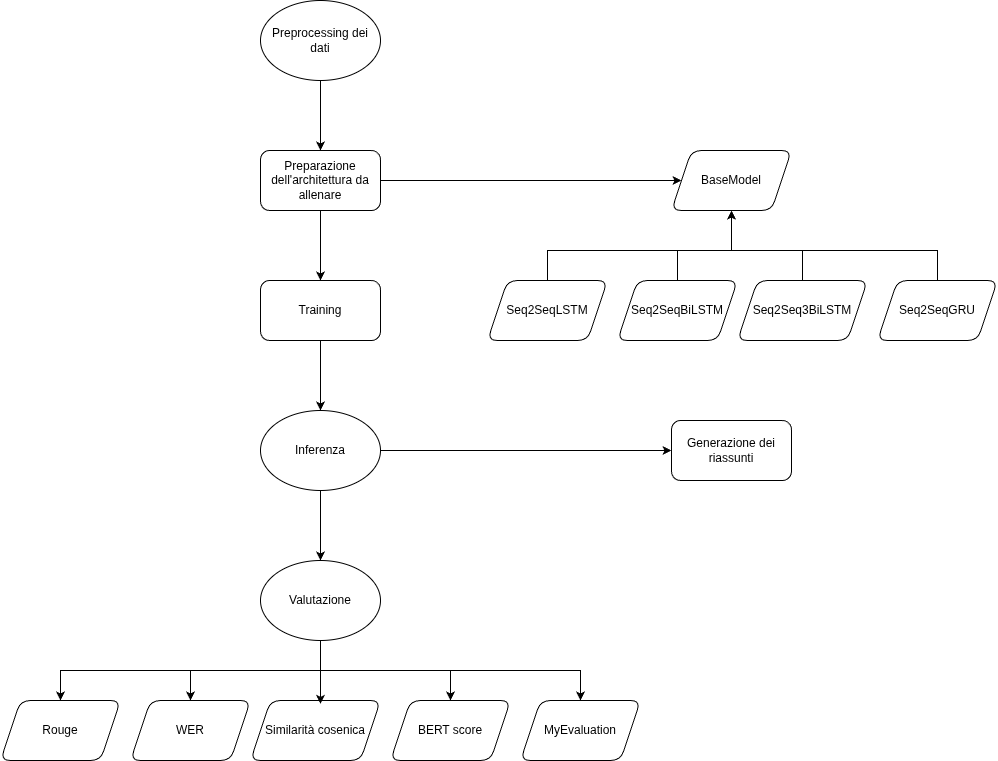
\includegraphics[width=1\textwidth]{media/pipeline.png}
    \caption{Pipeline del progetto}
    \label{fig:pipeline}
\end{figure}

The pipeline is divided into three main phases:
\begin{enumerate}
    \item \textbf{Preprocessing}: in this phase, data cleaning and preparation operations are performed, such as removing stopwords, tokenization, and text normalization.
    \item \textbf{Training}: in this phase, the summarization model is trained using the preprocessed data. A split is made between the training set and the validation set, and the model is trained using the training set while monitoring its performance on the validation set.
    \item \textbf{Evaluation}: in this phase, the summaries generated by the model are evaluated using various metrics, such as ROUGE, WER, BERT score, and the custom metric \texttt{myevaluation}.
\end{enumerate}
In the following sections, the details of each phase of the pipeline will be explored.
\section{Dataset}
Per questo progetto è stato utilizzato il dataset \href{https://www.kaggle.com/datasets/snap/amazon-fine-food-reviews}{SNAP Amazon Fine Food Reviews}, che contiene recensioni di prodotti alimentari di Amazon.\\
In particolare, il dataset contiene, per ogni riga, una recensione completa e il rispettivo riassunto.\\
Del dataset originale, composto da circa 500.000 righe, è stato selezionato un sottoinsieme di 10.000 righe per l'analisi e l'allenamento del modello.


\section{Preprocessing dei Dati}
Il preprocessing dei dati è una fase critica per garantire la qualità e l'efficacia dei modelli di summarization, infatti è fondamentale pulire e filtrare i dati in modo accurato.\\
Sul dataset, per l'appunto, sono stati eseguiti diversi passaggi di pulizia e filtraggio dei dati per garantire qualità e coerenza del modello durante l'addestramento.\\
Vediamo di seguito gli step effettutati durante questa fase:
\subsection{Pulizia del Testo}
Sono stati applicati i seguenti step di preprocessing:

\begin{enumerate}
    \item \textbf{Conversione del testo in minuscolo}
    \begin{itemize}
        \item Questa conversione garantisce l'uniformità del testo, evitando che la stessa parola venga considerata diversa solo per la presenza di maiuscole.\\Ad esempio, "Home", "HOME" e "home" vengono trattate come la stessa parola, riducendo la dimensionalità del vocabolario e migliorando l'efficienza dell'addestramento.
    \end{itemize}

    \item \textbf{Rimozione dei tag HTML}
    \begin{itemize}
        \item Le recensioni potrebbero contenere tag HTML residui dal formato web originale. 
        Questi elementi non contribuiscono al significato semantico del testo e potrebbero interferire con l'apprendimento del modello, pertanto vengono rimossi.
    \end{itemize}

    \item \textbf{Espansione delle contrazioni}
    \begin{itemize}
        \item Le contrazioni nella lingua inglese (come "don't", "I'm", "we're") vengono espanse nelle loro forme complete ("do not", "I am", "we are").\\
        Questo processo vuole standardizzare e garantire coerenza in tutto il testo e aiuta il modello a catturare meglio le relazioni semantiche, eliminando variazioni non necessarie della stessa espressione.
    \end{itemize}

    \item \textbf{Rimozione del genitivo sassone ('s)}
    \begin{itemize}
        \item La forma possessiva in inglese non altera sostanzialmente il significato della frase ai fini del riassunto.\\ 
        La sua rimozione semplifica il testo e riduce ulteriormente la dimensione del vocabolario, permettendo al modello di concentrarsi sui concetti principali.
    \end{itemize}

    \item \textbf{Eliminazione del testo tra parentesi}
    \begin{itemize}
        \item Il testo tra parentesi spesso contiene informazioni supplementari che non sono generalmente essenziali per il riassunto.\\ 
        La rimozione aiuta a mantenere il focus sulle informazioni principali della recensione.
    \end{itemize}

    \item \textbf{Rimozione della punteggiatura e caratteri speciali}
    \begin{itemize}
        \item La punteggiatura e i caratteri speciali, pur essendo importanti per la leggibilità umana, possono introdurre rumore nell'addestramento del modello.\\
        La rimozione semplifica il testo mantenendo intatto il contenuto semantico essenziale per la generazione del riassunto.
    \end{itemize}

    \item \textbf{Eliminazione delle stopwords}
    \begin{itemize}
        \item Le stopwords sono parole molto comuni (come "the", "is", "at", "which") che appaiono frequentemente ma portano poco significato semantico.\\
        La loro rimozione riduce significativamente la dimensionalità del problema senza perdere informazioni cruciali per il riassunto, permettendo al modello di concentrarsi sulle parole più significative.
    \end{itemize}

    \item \textbf{Rimozione delle parole troppo corte}
    \begin{itemize}
        \item Le parole molto corte (solitamente di una o due lettere) spesso non contribuiscono al significato del testo.\\
        La loro rimozione aiuta a ridurre ulteriormente il rumore nei dati, mantenendo solo i termini più significativi per l'analisi.
    \end{itemize}
\end{enumerate}

\subsection{Filtraggio dei Dati}
Dopo l'analisi statistica del dataset, sono stati applicati i seguenti vincoli:
\begin{itemize}
    \item Lunghezza massima delle recensioni: 30 parole
    \item Lunghezza massima dei riassunti: 8 parole
\end{itemize}

Questi limiti sono stati determinati attraverso un'analisi statistica della distribuzione delle lunghezze nel dataset, come possiamo vedere nella figura \ref{fig:dataset_length_distribuition}.
\begin{figure}[H]
    \centering
    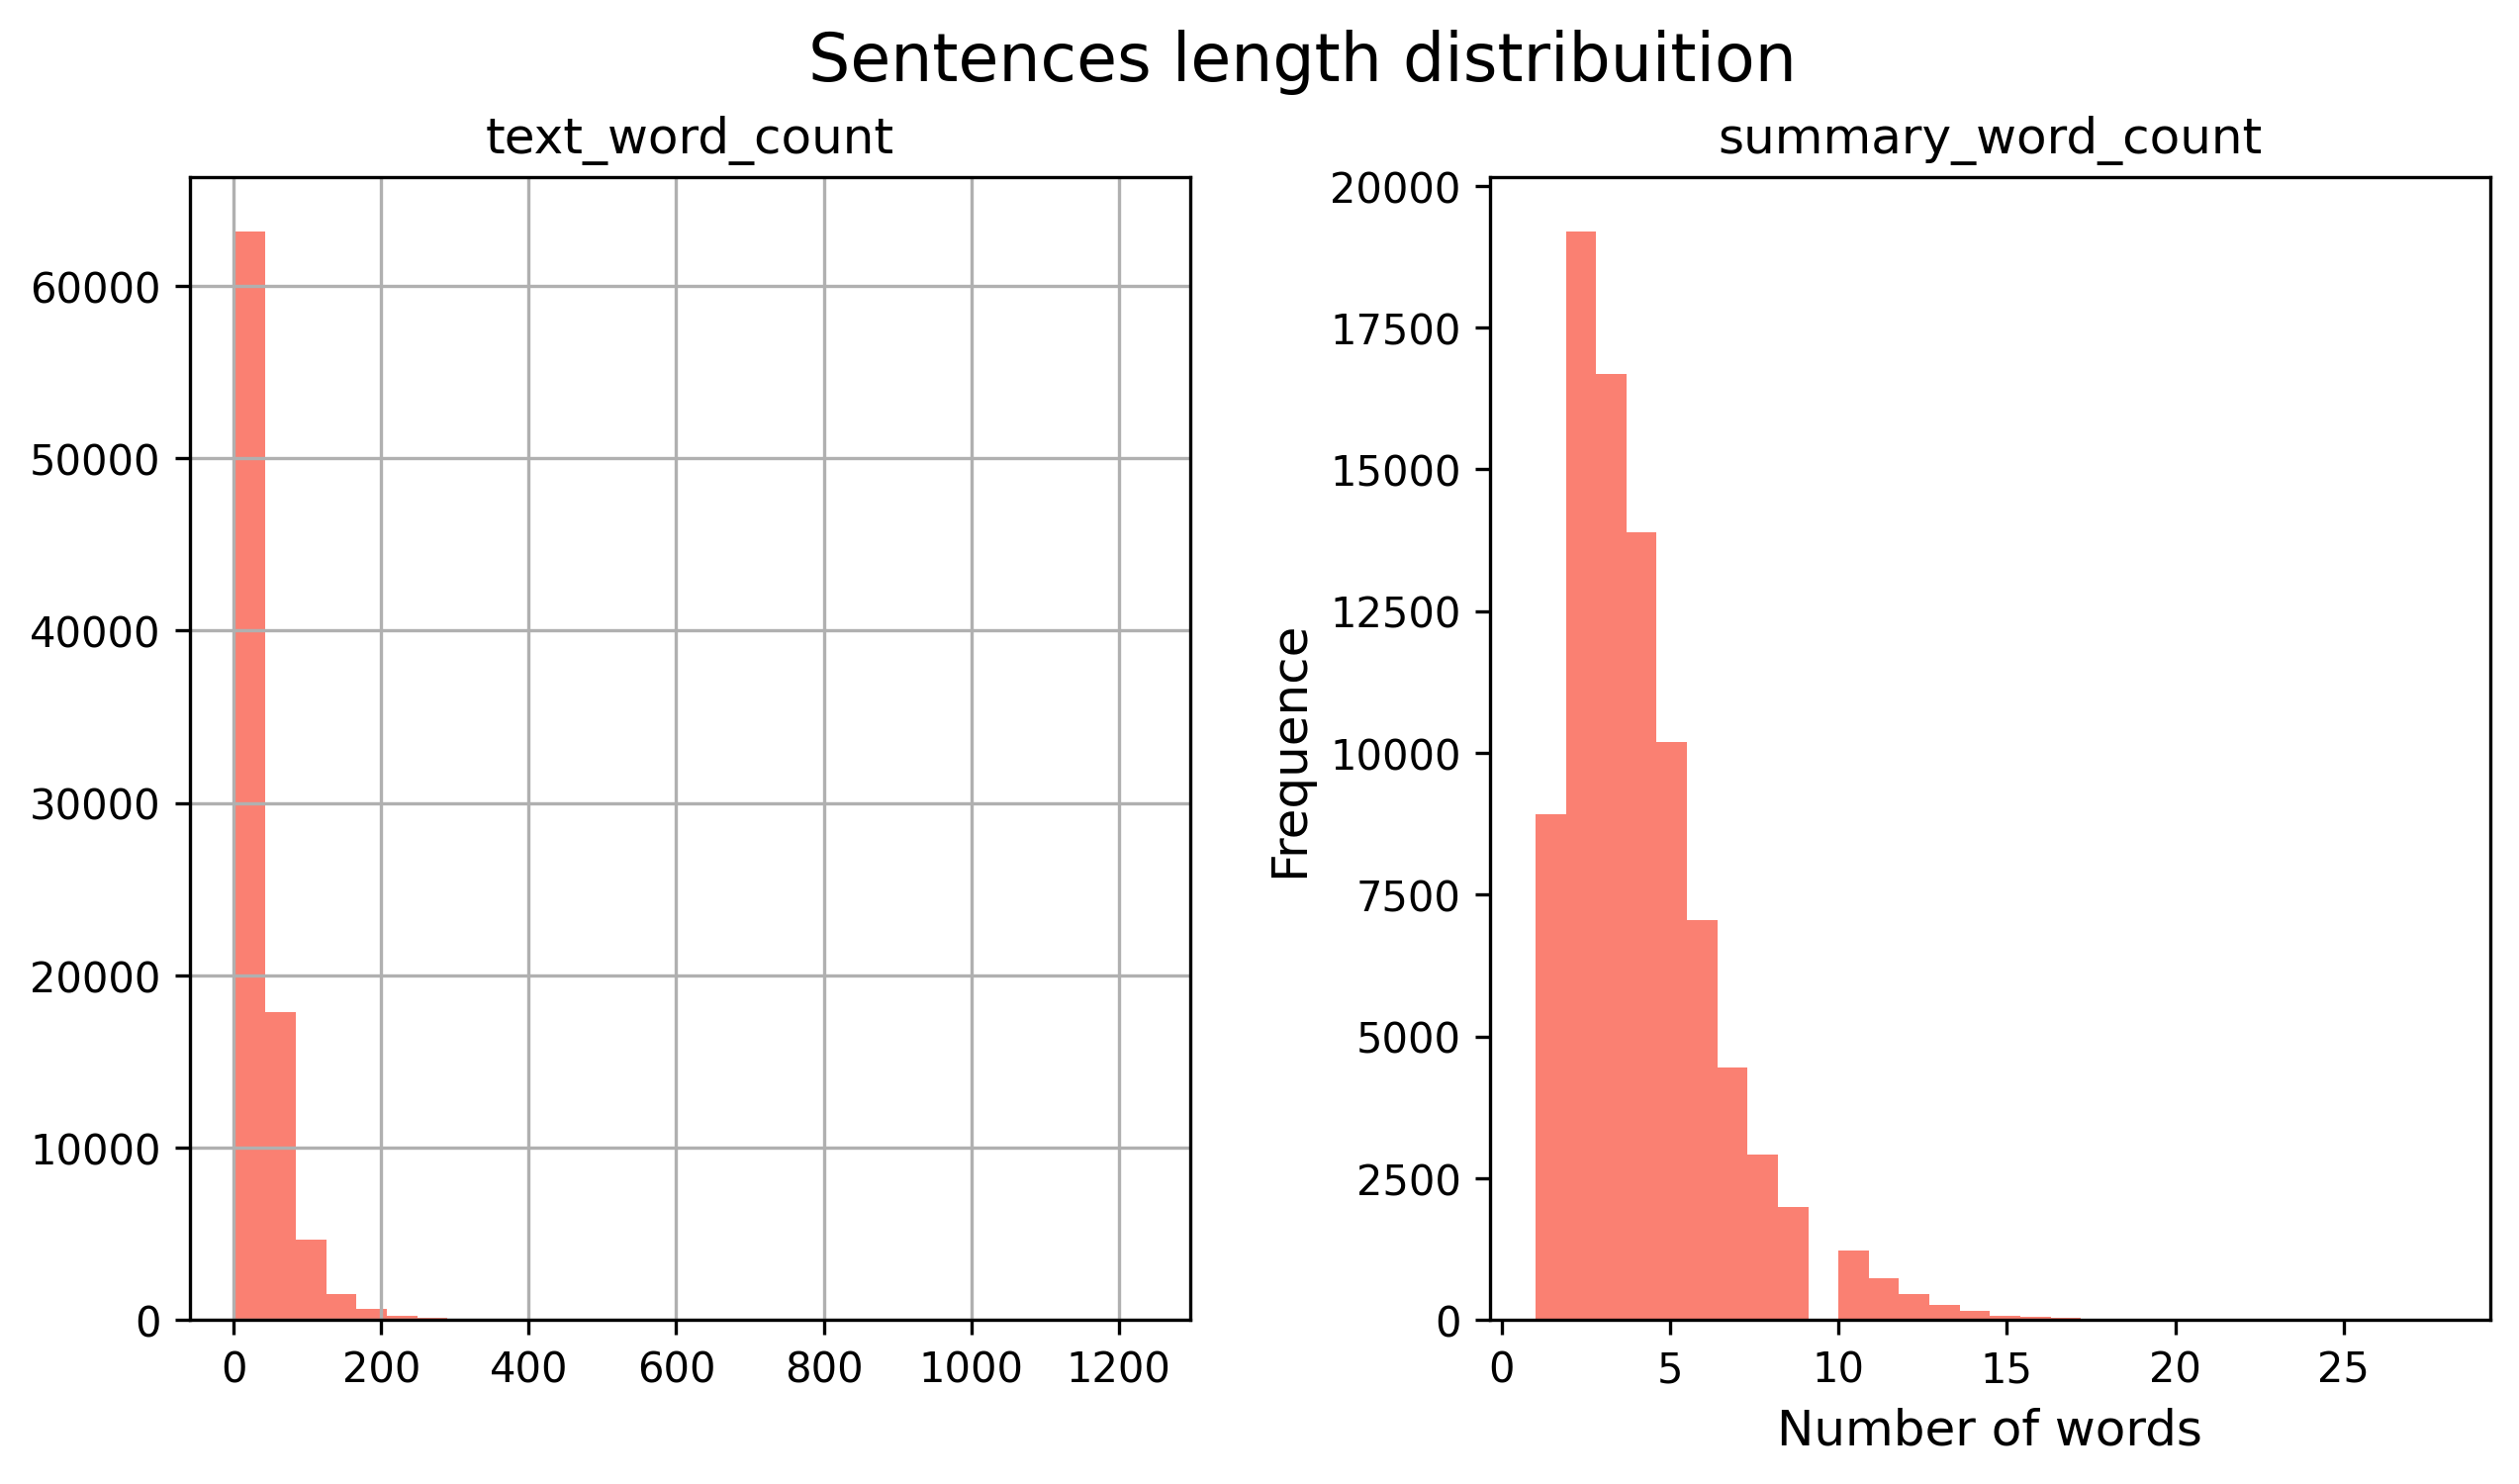
\includegraphics[width=1\textwidth]{media/dataset_length_distribuition.png}
    \caption{A sinistra la distribuzione delle lunghezze delle recensioni, a destra la distribuzione delle lunghezze dei riassunti}
    \label{fig:dataset_length_distribuition}
\end{figure}
Infatti, come si può notare dai due grafici, la maggior parte delle recensioni e dei riassunti ha lunghezze inferiori ai limiti stabiliti, quindi questi vincoli permettono di mantenere la maggior parte dei dati del dataset.

\subsection{Tokenizzazione e Token Speciali}
Per preparare i dati per i modelli ho aggiunto i token speciali \texttt{"sostok"} e \texttt{"eostok"} per indicare l'inizio e la fine di una sequenza, in modo da facilitare la tokenizzazione e la fase di addestramento.\\
Inoltre, ho effettuato la tokenizzazione separatamente per le recensioni (testo di input) e i riassunti (testo di output) per garantire che il modello possa apprendere correttamente la relazione tra i due.
I due tokenizer servono a creare il vocabolario per le recensioni e per i riassunti, in modo da poter convertire i testi in sequenze di token.

\definecolor{lightgray}{gray}{0.95}

\newcommand{\risultati}[4]{
  \subsubsection{Results}
  This model achieved the following results at the end of training:
  \begin{table}[H]
  \centering
  \rowcolors{2}{lightgray}{white}
  \begin{tabular}{@{} >{\bfseries}l c @{}}
    \toprule
    \textbf{Metric}    & \textbf{Value} \\
    \midrule
    Loss                & #1              \\
    Validation Loss     & #2              \\
    Accuracy            & #3              \\
    Validation Accuracy & #4              \\
    \bottomrule
  \end{tabular}
  \caption{Results of the model at the end of training}
  \label{tab:risultati}
  \end{table}
}

\newcommand{\training}[8]{
  \subsubsection{Training}
  The training of the model was carried out using the following configuration:
  \begin{table}[ht]
    \centering
    \rowcolors{2}{lightgray}{white}
    \begin{tabular}{@{} >{\bfseries}l c @{}}
      \toprule
      \textbf{Parameter}        & \textbf{Value} \\
      \midrule
      Optimizer                 & #1              \\
      Learning rate             & #2              \\
      Embedding dimension       & #3              \\
      Latent dimension          & #4              \\
      Decoder dropout           & #5              \\
      Decoder recurrent dropout & #6              \\
      Encoder dropout           & #7              \\
      Encoder recurrent dropout & #8              \\
      \trainingcontinued
      }

      \newcommand{\trainingcontinued}[2]{
      Batch size                & #1              \\
      Epochs                    & #2              \\
      \bottomrule
    \end{tabular}
    \caption{Training configuration}
  \end{table}

  \lossimg
}

\newcommand{\lossimg}[2]{
  We can check the trend of the losses during training in Figure \ref{fig:#2}.

  \begin{figure}[H]
    \centering
    \includegraphics[width=0.75\textwidth]{media/#1_best_lossplot.png}
    \caption{Trend of the \textit{loss} and \textit{validation loss} during training}
    \label{fig:#2}

  \end{figure}
}

\newcommand{\architecture}[3]{
  \subsubsection{Architecture}
  The architecture used is as follows:
  \archimg{#1}{#2}{#3}
}

\newcommand{\archimg}[3]{
  \begin{figure}[H]
    \centering
    \includegraphics[width=0.75\textwidth]{media/#1_best_architecture.png}
    \caption{Architecture of the model #2}
    \label{fig:#3}
  \end{figure}
}

\newcommand{\rougeonesubimg}[3]{
  \begin{subfigure}{#1\textwidth}
    \centering
    \includegraphics[width=\textwidth]{media/#2_best_rouge1_scores.png}
    \caption{ROUGE-1 #2}
    \label{fig:#3}
  \end{subfigure}
}

\newcommand{\rougetwosubimg}[3]{
  \begin{subfigure}{#1\textwidth}
    \centering
    \includegraphics[width=\textwidth]{media/#2_best_rouge2_scores.png}
    \caption{ROUGE-2 #2}
    \label{fig:#3}
  \end{subfigure}
}

\newcommand{\rougelubimg}[3]{
  \begin{subfigure}{#1\textwidth}
    \centering
    \includegraphics[width=\textwidth]{media/#2_best_rougeL_scores.png}
    \caption{ROUGE-L #2}
    \label{fig:#3}
  \end{subfigure}
}

\newcommand{\wersubimg}[3]{
  \begin{subfigure}{#1\textwidth}
    \centering
    \includegraphics[width=\textwidth]{media/#2_best_wer_scores.png}
    \caption{WER #2}
    \label{fig:#3}
  \end{subfigure}
}

\newcommand{\cssubimg}[3]{
  \begin{subfigure}{#1\textwidth}
    \centering
    \includegraphics[width=\textwidth]{media/#2_best_cosine_similarity_scores.png}
    \caption{Cosine similarity #2}
    \label{fig:#3}
  \end{subfigure}
}

\newcommand{\bertsubimg}[3]{
  \begin{subfigure}{#1\textwidth}
    \centering
    \includegraphics[width=\textwidth]{media/#2_best_bert_scores.png}
    \caption{BERT score #2}
    \label{fig:#3}
  \end{subfigure}
}

\newcommand{\myevalsubimg}[3]{
  \begin{subfigure}{#1\textwidth}
    \centering
    \includegraphics[width=\textwidth]{media/#2_best_myevaluation_scores.png}
    \caption{My Evaluation #2}
    \label{fig:#3}
  \end{subfigure}
}

\section{Architettura dei Modelli}
Per svolgere questo progetto ho deciso di effettuare un confronto tra diversi modelli, implementando architetture \textbf{Sequence to Sequence} con \textbf{LSTM} e \textbf{GRU}.\\
L'implementazione dei modelli è stata effettuata attraverso una classe astratta \texttt{BaseModel} e la successiva creazioni e implementazione di classi derivate.\\
Questo permette di definire un'interfaccia comune per tutti i modelli di summarization e di estendere facilmente l'architettura in futuro.\\

\subsection{Classe Base Astratta}
La classe \texttt{BaseModel} fornisce l'interfaccia base per tutti i modelli di summarization:
\begin{itemize}
    \item Metodi astratti per costruire encoder e decoder.
    \item Funzionalità per il salvataggio, caricamento e inferenza del modello.
    \item Conversione tra sequenze di token e testo tramite i tokenizer.
\end{itemize}

\subsection{Training}
L'addestramento dei modelli, derivati dalla classe \texttt{BaseModel}, è stato effettuato utilizzando il dataset preprocessato.\\
Prima di iniziare l'addestramento, il dataset è stato suddiviso in training set e validation set, con una proporzione del 90\% e 10\% rispettivamente.\\
Dopodiché sono passato alla fase effettiva di training dei modelli, utilizzando e la funzione loss \texttt{Sparse Categorical Crossentropy}, utile nei task di summarization.\\

\subsection{Iperparametri}
Per ogni classe di modello, il training è stato eseguito più volte, ciascuna con una combinazione diversa di iperparametri.\\
Queste combinazioni vengono generate tramite una \textit{hyperparameter\_grid}
implementata nella funzione \texttt{create\_hyperparameter\_grid}, che restituisce tutte le
permutazioni possibili tra i valori forniti per i seguenti parametri:
\begin{itemize}
    \item \texttt{embedding\_dim}: dimensione dell'embedding delle parole
    \item \texttt{hidden\_dim}: dimensione dello stato nascosto dell'encoder e del decoder
    \item \texttt{encoder\_dropout}: tasso di dropout dell'encoder
    \item \texttt{encoder\_recurrent\_dropout}: tasso di dropout per gli stati ricorrenti dell'encoder
    \item \texttt{decoder\_dropout}: tasso di dropout del decoder
    \item \texttt{decoder\_recurrent\_dropout}: tasso di dropout per gli stati ricorrenti del decoder
    \item \texttt{optimizer}: ottimizzatore da utilizzare durante l'addestramento
    \item \texttt{learning\_rate}: tasso di apprendimento
    \item \texttt{batch\_size}: dimensione del batch durante l'addestramento
    \item \texttt{epochs}: numero di epoche per l'addestramento
\end{itemize}

Per ogni \textbf{permutazione} di iperparametri, viene eseguito il seguente processo di allenamento:
\begin{enumerate}
    \item \textbf{Preparazione dei dati}: viene eseguita la parte di caricamento e preprocessing dei dati
    \item \textbf{Istanza del modello}: viene istanziata la classe del modello corrento con gli iperparametri selezionati
    \item \textbf{Training del modello}: viene eseguito il training del modello con alcune callback, di cui verrà parlato in seguito
    \item \textbf{Salvataggio dei risultati}:
          \begin{itemize}
              \item \textit{Pesi del modello} (\texttt{result/\{model\_class\}/weights/})
              \item \textit{Architettura del modello} (\texttt{result/\{model\_class\}/media/architectures/})
              \item \textit{Grafico dell'andamento della loss} (\texttt{result/\{model\_class\}/media/graphs/})
              \item \textit{Cronologia dell'allenamento} (\texttt{result/\{model\_class\}/histories/})
              \item \textit{Riassunti generati}: al termine del training vengono generati i riassunti, partendo da recensioni presenti nel validation set, e salvati in un file csv (\texttt{result/\{model\_class\}/csv/})
          \end{itemize}
\end{enumerate}

\subsubsection{Callback}
Durante il training ho utilizzato anche le seguenti funzioni di callback:
\begin{itemize}
    \item \textbf{Early Stopping}: monitora una metrica, in questo caso la validation loss, e interrompe l'addestramento se non ci sono miglioramenti per un certo numero di epoche consecutive. Questo aiuta a prevenire l'overfitting e a risparmiare tempo di calcolo.
    \item \textbf{Learning Rate Scheduler}: regola il tasso di apprendiento durante il training secondo una strategia, nel mio caso ho utilizzato la \texttt{Step Decay}, che riduce il learning rate di un fattore fisso ogni tot epoche.
    \item \textbf{Reduce LR on Plateau}: monitora una metrica, in questo caso la validation loss, e riduce il learning rate se non ci sono miglioramenti per un certo numero di epoche consecutive. Questo aiuta a ottimizzare il processo di addestramento e a trovare un tasso di apprendimento più efficace.
\end{itemize}
In questo modo sono riuscito a ottenere i risultati migliori per ogni modello, aggiustando i suoi iperparametrie e provando le diverse combinazioni.

\subsection{Architetture Sperimentate}
Sono state sperimentante diverse architetture di modelli di summarization, ognuna con caratteristiche e parametri diversi.\\
Le due categorie principali di modelli implementati sono:
\begin{itemize}
    \item \textbf{LSTM}: modelli basati su layer LSTM per encoder e decoder.
    \item \textbf{GRU}: modelli basati su layer GRU per encoder e decoder.
\end{itemize}
Tali architetture sono basate sulle RNN (Recurrent Neural Networks) e sono state scelte per la loro efficacia nei task di text-summarization, poiché
gestiscono le dipendenze tra le parole su sequenze di testo.\\
\begin{itemize}
    \item \textbf{LSTM}: Long Short-Term Memory, è una variante delle RNN che risolve il problema della scomparsa del gradiente, grazie alla presenza di un meccanismo di memoria a lungo termine.
          Tale meccanismo di gating permette di memorizzare informazioni importanti e scartare quelle meno rilevanti.
    \item \textbf{GRU}: Gated Recurrent Unit, è una variante più semplice delle LSTM, con meno parametri e meno complessità computazionale.
          Anche in questo caso, il meccanismo di gating permette di memorizzare informazioni importanti e scartare quelle meno rilevanti.
\end{itemize}

Al fine di rendere più scorrevole la lettura, per ogni classe vengono riportati solamente i migliori risultati ottenuti durante l'addestramento con i migliori parametri e le migliori configurazioni trovate (basate sul \texttt{BERTScore}, di cui verrà parlato in seguito), sebbene
siano stati effettuati numerosi tentativi e test riportati nelle prossime sezioni in una tabella comparativa.\\


\subsection{Seq2SeqLSTM}
The \texttt{Seq2SeqLSTM} class implements the specific architecture for the Sequence to Sequence summarization model with LSTM layers.

\training{Adam}{0.001}{512}{128}{0.2}{0.2}{0.2}{0.2}{128}{50}{Seq2SeqLSTM}{seq2seqlstm_loss_plot}
\risultati{1.63}{2.02}{0.67}{0.64}
\architecture{Seq2SeqLSTM}{Seq2SeqLSTM}{seq2seqlstm_architecture}

\subsection{Seq2SeqBiLSTM}
La classe \texttt{Seq2SeqBiLSTM} implementa un'architettura simile al modello Seq2SeqLSTM, ma i layer LSTM dell'encoder sono bidirezionali.

\training{Adam}{0.001}{512}{256}{0.2}{0.2}{0.2}{0.2}{64}{50}{Seq2SeqBiLSTM}{seq2seqbilstm_loss_plot}
\risultati{1.23}{2.01}{0.72}{0.65}
\architecture{Seq2SeqBiLSTM}{Seq2SeqBiLSTM}{seq2seqbilstm_architecture}
\subsection{Seq2Seq3BiLSTM}
The \texttt{Seq2Seq3BiLSTM} class implements an architecture similar to the Seq2SeqBiLSTM model, but with three bidirectional LSTM layers in the encoder.

\training{Adam}{0.001}{256}{256}{0.2}{0.2}{0.2}{0.2}{128}{50}{Seq2Seq3BiLSTM}{seq2seq3bilstm_loss_plot}
\risultati{1.51}{1.99}{0.68}{0.65}
\architecture{Seq2Seq3BiLSTM}{Seq2Seq3BiLSTM}{seq2seq3bilstm_architecture}
%\subsection{Seq2SeqLSTMGloVe}
La classe \texttt{Seq2SeqLSTMGloVe} implementa un'architettura simile al modello Seq2SeqLSTM, utilizzando i vettori di embedding GloVe preaddestrati per la rappresentazione delle parole.\\
Più precisamente vengono scaricati e utilizzati i vettori di embedding GloVe preaddestrati da \href{https://nlp.stanford.edu/projects/glove/}{Stanford NLP Group} da 100 dimensioni, anche se la classe consente di scambiare facilmente i vettori con quelli di dimensione diversa.\\

\training{Adam}{50}
\risultati{DA INSERIRE}{DA INSERIRE}{DA INSERIRE}{DA INSERIRE}
Possiamo verifcare l'andamento delle loss durante l'addestramento nella figura \ref{fig:seq2seqlstmglove_loss_plot}.
\begin{figure}[H]
    \centering
    \includegraphics[width=0.75\textwidth]{media/Seq2SeqLSTMGloVe_originale_lossplot.png}
    \caption{Andamento delle loss durante l'addestramento}
    \label{fig:seq2seqlstmglove_loss_plot}
\end{figure}

\subsection{Seq2SeqGRU}
La classe \texttt{Seq2SeqGRU} implementa un'architettura Seq2Seq con GRU, utilizzando layer GRU per l'encoder e il decoder.
\training{Adam}{0.001}{256}{128}{0.2}{0.2}{0.2}{0.2}{128}{50}{Seq2SeqGRU}{seq2seqgru_loss_plot}
\risultati{1.58}{2.01}{0.67}{0.64}
\architecture{Seq2SeqGRU}{Seq2SeqGRU}{seq2seqgru_architecture}
\section{Evaluation Metrics}
In this section, the performance of the models is analyzed through the graphs of the main evaluation metrics: ROUGE \cite{lin-2004-rouge}, cosine similarity, and BERT score \cite{zhang2020bertscoreevaluatingtextgeneration}.\\
Additionally, a custom metric \texttt{myevaluation} was also used, which will be discussed later.\\
These metrics were chosen to accurately measure the quality of the generated summaries by comparing them with the reference summaries.\\
The evaluations were conducted using the test dataset, which was not used during the model training phase.\\

\subsection{Evaluation by Permutation}
For each permutation of architectures and their respective hyperparameters,
a structured evaluation process was followed at the end of the
training phase. Below are the evaluation metrics used.

\subsection{ROUGE (Recall-Oriented Understudy for Gisting Evaluation)}
Three variants of ROUGE were calculated:
\begin{itemize}
    \item ROUGE-1: compares unigrams between the generated summary and the reference summary
    \item ROUGE-2: considers bigrams to evaluate the similarity between the two texts
    \item ROUGE-L: compares the longest common subsequence between the two texts
\end{itemize}

The graphs in Figure \ref{fig:rouge_comparison} compare the performance in terms of ROUGE-1, ROUGE-2, and ROUGE-L for the four models. The Seq2SeqBiLSTM model shows an improvement in ROUGE scores compared to Seq2SeqLSTM, Seq2Seq3BiLSTM, and Seq2SeqGRU, indicating a greater ability to capture lexical similarities.
\begin{figure}[H]
    \centering
    \rougeonesubimg{0.45}{Seq2SeqLSTM}{rouge1_seq2seq_lstm}
    \hfill
    \rougeonesubimg{0.45}{Seq2SeqBiLSTM}{rouge1_seq2seq_bilstm}
    \hfill
    \rougeonesubimg{0.45}{Seq2Seq3BiLSTM}{rouge1_seq2seq_3bilstm}
    \hfill
    %\rougeonesubimg{0.45}{Seq2SeqLSTMGlove}{rouge1_seq2seq_lstm_glove}
    %\hfill
    \rougeonesubimg{0.45}{Seq2SeqGRU}{rouge1_seq2seq_gru}
    \hfill

    \rougetwosubimg{0.45}{Seq2SeqLSTM}{rouge2_seq2seq_lstm}
    \hfill
    \rougetwosubimg{0.45}{Seq2SeqBiLSTM}{rouge2_seq2seq_bilstm}
    \hfill
    \rougetwosubimg{0.45}{Seq2Seq3BiLSTM}{rouge2_seq2seq_3bilstm}
    \hfill
    %\rougetwosubimg{0.45}{Seq2SeqLSTMGlove}{rouge2_seq2seq_lstm_glove}
    %\hfill
    \rougetwosubimg{0.45}{Seq2SeqGRU}{rouge2_seq2seq_gru}
    \hfill

    \rougelubimg{0.45}{Seq2SeqLSTM}{rougeL_seq2seq_lstm}
    \hfill
    \rougelubimg{0.45}{Seq2SeqBiLSTM}{rougeL_seq2seq_bilstm}
    \hfill
    \rougelubimg{0.45}{Seq2Seq3BiLSTM}{rougeL_seq2seq_3bilstm}
    \hfill
    %\rougelubimg{0.45}{Seq2SeqLSTMGlove}{rougeL_seq2seq_lstm_glove}
    %\hfill
    \rougelubimg{0.45}{Seq2SeqGRU}{rougeL_seq2seq_gru}
    \hfill

    \caption{ROUGE scores comparison between Seq2SeqLSTM, Seq2SeqBiLSTM, Seq2Seq3BiLSTM and Seq2SeqGRU architectures.}
    \label{fig:rouge_comparison}
\end{figure}

% \subsection{WER (Word Error Rate)}
% The WER is a metric that calculates the error rate between two sequences of words.\\
% In particular, the WER calculates the number of insertion, deletion, and substitution operations needed to transform one word sequence into another.\\

% The WER comparison, shown in Figure \ref{fig:wer_comparison}, highlights that the Seq2Seq3BiLSTM model achieves better results, indicating a greater accuracy in word generation, although the difference with the Seq2SeqBiLSTM architecture is not significant.\\

% \begin{figure}[H]
%     \centering
%     \wersubimg{0.45}{Seq2SeqLSTM}{wer_seq2seq_lstm}
%     \hfill
%     \wersubimg{0.45}{Seq2SeqBiLSTM}{wer_seq2seq_bilstm}
%     \hfill
%     \wersubimg{0.45}{Seq2Seq3BiLSTM}{wer_seq2seq_3bilstm}
%     \hfill
%     %\wersubimg{0.45}{Seq2SeqLSTMGlove}{wer_seq2seq_lstm_glove}
%     %\hfill
%     \wersubimg{0.45}{Seq2SeqGRU}{wer_seq2seq_gru}

%     \caption{WER scores comparison between Seq2SeqLSTM, Seq2SeqBiLSTM, Seq2Seq3BiLSTM and Seq2SeqGRU architectures.}
%     \label{fig:wer_comparison}
% \end{figure}


\subsection{Cosine Similarity}
Cosine similarity is a metric that calculates the similarity between two vectors in a multidimensional space.\\
In the specific case of summary generation, cosine similarity was calculated between the embedding vectors of the words in the generated summaries and those in the reference summaries, in order to evaluate the quality of the generated summaries.\\
Figure \ref{fig:cosine_similarity_comparison} compares the cosine similarity values. Again, the Seq2SeqBiLSTM model achieves higher values, suggesting a greater semantic correlation with the reference summaries.

\begin{figure}[H]
    \centering
    \cssubimg{0.45}{Seq2SeqLSTM}{cs_seq2seq_lstm}
    \hfill
    \cssubimg{0.45}{Seq2SeqBiLSTM}{cs_seq2seq_bilstm}
    \hfill
    \cssubimg{0.45}{Seq2Seq3BiLSTM}{cs_seq2seq_3bilstm}
    \hfill
    %\cssubimg{0.45}{Seq2SeqLSTMGlove}{cs_seq2seq_lstm_glove}
    %\hfill
    \cssubimg{0.45}{Seq2SeqGRU}{cs_seq2seq_gru}

    \caption{Cosine similarity scores comparison between Seq2SeqLSTM, Seq2SeqBiLSTM, Seq2Seq3BiLSTM and Seq2SeqGRU architectures.}
    \label{fig:cosine_similarity_comparison}
\end{figure}

\subsection{BERT Score}
BERT score is a metric that uses the BERT model to calculate the similarity between two texts.\\
In particular, BERT score calculates the similarity between the embedding vectors of the words in the generated summaries and those in the reference summaries, taking into account the semantic context of the words.\\
Figure \ref{fig:bert_score_comparison} shows the BERT score values for the different models. Again, the Seq2SeqBiLSTM model achieves better results, suggesting a greater ability to capture the semantic similarity between the generated summaries and the reference ones.

\begin{figure}[H]
    \centering
    \bertsubimg{0.45}{Seq2SeqLSTM}{bert_seq2seq_lstm}
    \hfill
    \bertsubimg{0.45}{Seq2SeqBiLSTM}{bert_seq2seq_bilstm}
    \hfill
    \bertsubimg{0.45}{Seq2Seq3BiLSTM}{bert_seq2seq_3bilstm}
    \hfill
    %\bertsubimg{0.45}{Seq2SeqLSTMGlove}{bert_seq2seq_lstm_glove}
    %\hfill
    \bertsubimg{0.45}{Seq2SeqGRU}{bert_seq2seq_gru}
    \hfill

    \caption{BERT score comparison between Seq2SeqLSTM, Seq2SeqBiLSTM, Seq2Seq3BiLSTM and Seq2SeqGRU architectures.}
    \label{fig:bert_score_comparison}
\end{figure}

\subsection{My Evaluation}
The \texttt{myevaluation} metric was designed to evaluate the quality of the generated summaries in a more detailed way.\\
It takes into account several factors, each of which has a specific weight based on its importance.\\
The formula used to calculate the \texttt{myevaluation} metric is as follows:
\[
    \texttt{MyEval} = cs\_PS\_OS \cdot W_{cs\_PS\_OS} + keyword\_overlap \cdot W_{keyword\_overlap} + bert\_score \cdot W_{bert\_score}
\]
Where:
\begin{itemize}
    \item $cs\_PS\_OS$ is the cosine similarity between the generated summary and the original one
    \item $keyword\_overlap$ is the percentage of keywords present in the generated summary compared to those in the original summary
    \item $bert\_score$ is the BERT score between the generated summary and the original one
    \item $W_{cs\_PS\_OS}$, $W_{keyword\_overlap}$ and $W_{bert\_score}$ are the weights associated with each factor
          \begin{itemize}
              \item $W_{cs\_PS\_OS} = 0.07$
              \item $W_{keyword\_overlap} = 0.03$
              \item $W_{bert\_score} = 0.9$
          \end{itemize}
\end{itemize}

Figure \ref{fig:myevaluation_comparison} shows the results of the \texttt{myevaluation} metric for the different models.\\
The Seq2SeqBiLSTM model achieves the highest scores, suggesting a superior quality of the generated summaries compared to the other models.
\begin{figure}[H]
    \centering
    \myevalsubimg{0.45}{Seq2SeqLSTM}{myeval_seq2seq_lstm}
    \hfill
    \myevalsubimg{0.45}{Seq2SeqBiLSTM}{myeval_seq2seq_bilstm}
    \hfill
    \myevalsubimg{0.45}{Seq2Seq3BiLSTM}{myeval_seq2seq_3bilstm}
    \hfill
    %\myevalsubimg{0.45}{Seq2SeqLSTMGlove}{myeval_seq2seq_lstm_glove}
    %\hfill
    \myevalsubimg{0.45}{Seq2SeqGRU}{myeval_seq2seq_gru}
    \hfill

    \caption{Comparison of the \texttt{myevaluation} metric between Seq2SeqLSTM, Seq2SeqBiLSTM, Seq2Seq3BiLSTM and Seq2SeqGRU architectures.}
    \label{fig:myevaluation_comparison}
\end{figure}

\subsection{Architectures Comparison}
Below is a comparative table (Figure \ref{fig:models_comparison_instances}) between the various implemented models, with their respective results obtained at the end of training.\\
For each model class, numerous attempts and tests were conducted, which are reported later in a comparative table of the various configuration instances and the results obtained.\\
We can immediately see that the Seq2SeqBiLSTM model achieved the best results in almost all metrics.
\begin{figure}[H]
    \centering
    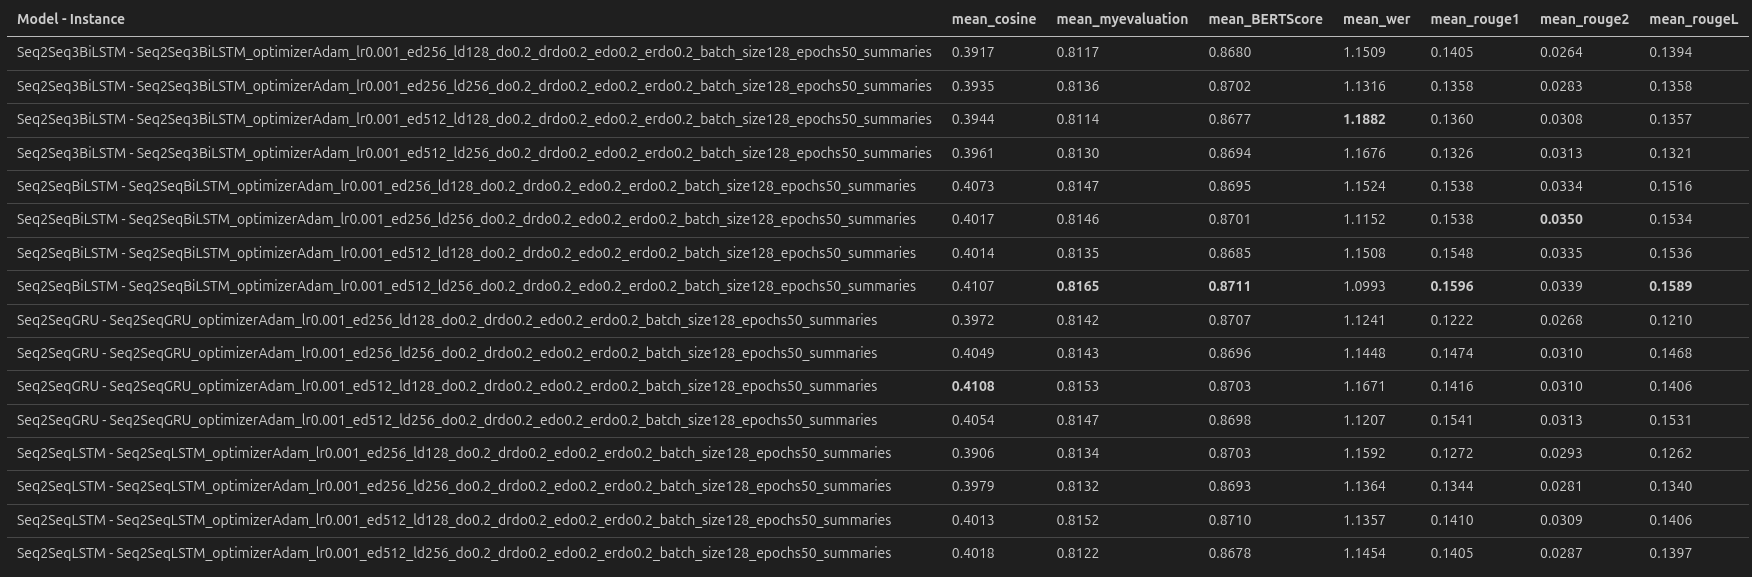
\includegraphics[width=1\textwidth]{media/models_comparison_instances.png}
    \caption{Comparative analysis of model instances}
    \label{fig:models_comparison_instances}
\end{figure}


\section{Conclusioni}
\subsection{Considerazioni Finali}
Il lavoro svolto ha portato allo sviluppo di un sistema di sintesi automatica in grado di generare riassunti coerenti a partire da recensioni di cibo. Il sistema è stato progettato per garantire facilità di estensione e adattabilità a diverse tipologie di task, aumentando così la sua versatilità e potenziale applicativo in contesti variegati.\\
Nel corso del progetto sono stati implementati diversi modelli di sintesi automatica, tra cui Seq2SeqLSTM, Seq2SeqBiLSTM, Seq2Seq3BiLSTM e Seq2SeqGRU.
I risultati sono stati valutati attraverso numerose metriche, quali ROUGE, Word Error Rate (WER), Cosine Similarity, BERTScore e \texttt{MyEvaluation}. In particolare,
la BERTScore si è rivelata la metrica più rappresentativa della qualità dei riassunti, in quanto considera il contesto semantico e la similarità delle parole.\\

Inoltre, la metrica \texttt{MyEvaluation} ha fornito una valutazione più dettagliata della qualità dei riassunti, integrando vari fattori e assegnando a ciascuno
un peso in base alla sua rilevanza. I risultati sperimentali indicano che il modello \textbf{Seq2SeqBiLSTM} ha ottenuto le prestazioni migliori su quasi tutte le metriche,
suggerendo una superiore capacità di catturare le similarità semantiche tra i riassunti generati e quelli di riferimento.
L'architettura \textbf{Seq2SeqBiLSTM} ha raggiunto risultati eccellenti, conseguendo su 1000 riassunti:
\begin{table}[ht]
    \centering
    \rowcolors{2}{lightgray}{white}
    \begin{tabular}{@{} >{\bfseries}l c @{}}
        \toprule
        \textbf{Metrica}    & \textbf{Valore} \\
        \midrule
        ROUGE-1             & 0.16            \\
        ROUGE-2             & 0.03            \\
        ROUGE-L             & 0.16            \\
        WER                 & 1.09            \\
        Similarità cosenica & 41\%            \\
        BERTScore           & 87\%            \\
        MyEvaluation        & 82\%            \\
        \bottomrule
    \end{tabular}
    \caption{Metriche di valutazione del modello}
\end{table}

È opportuno sottolineare che i risultati sono stati influenzati dalla scelta del dataset e dalle specifiche caratteristiche dei dati,
inclusi gli aspetti relativi al preprocessing. Tali elementi evidenziano l'importanza di un'attenta selezione e preparazione dei dati per
ottimizzare le prestazioni dei modelli di sintesi automatica.

\subsection{Test del Modello Migliore}
Il modello \textbf{Seq2SeqBiLSTM} ha mostrato prestazioni superiori rispetto agli altri modelli implementati.\\
Di seguito vengono riportati alcuni esempi di sintesi generate dal modello \textbf{Seq2SeqBiLSTM} e i rispettivi testi e riassunti di riferimento.\\

\begin{figure}[H]
    \centering
    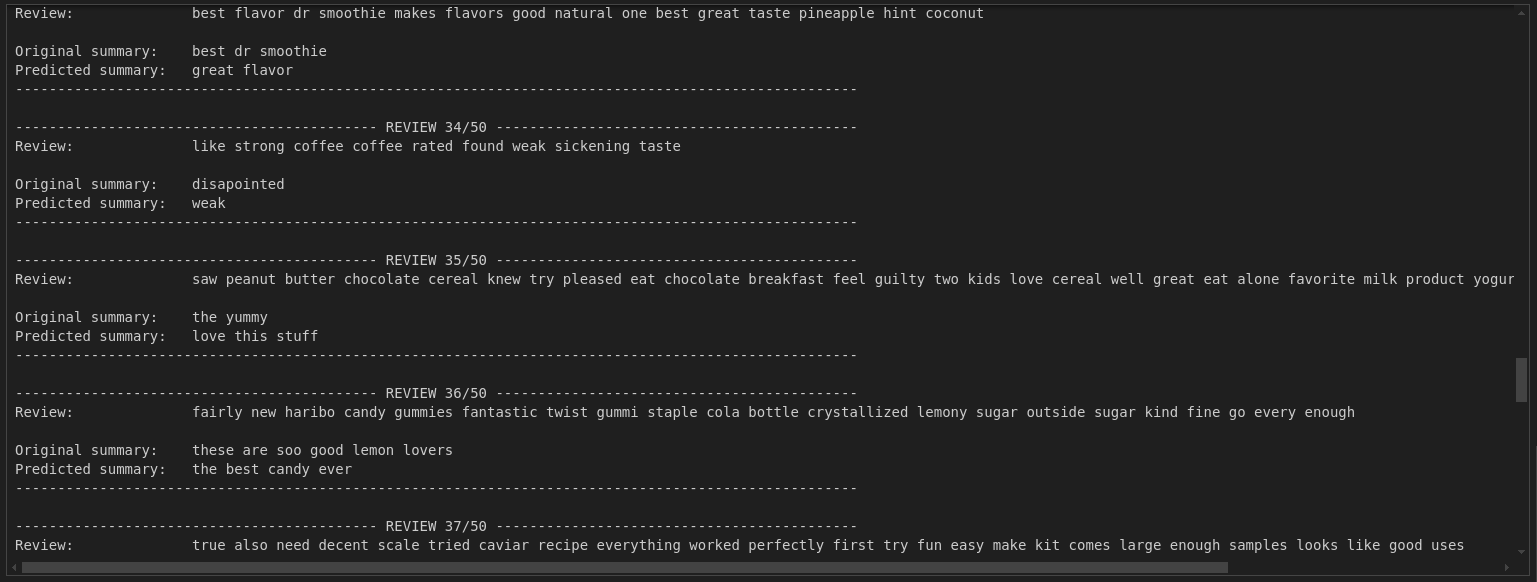
\includegraphics[width=0.75\textwidth]{media/Seq2SeqBiLSTM_inference.png}
    \caption{Esempio di sintesi generata dal modello Seq2SeqBiLSTM}
    \label{fig:example1}
\end{figure}

\newpage
\printbibliography

\end{document}